\documentclass[10pt]{beamer}
\usepackage{amsmath,amssymb,longtable,hhline}
\usepackage{mathrsfs}
\usepackage{xcolor}
\usepackage{hyperref}
\usepackage{multicol}
\usepackage{anyfontsize}
\usepackage{minted}
\usepackage{alltt}
\usepackage{fontawesome}

\usemintedstyle{tango}
\newcommand{\ltprgsize}{\fontsize{5}{5}\selectfont}
%\newcommand{\ltprgsize}{\footnotesize}
\setminted{fontsize=\footnotesize,mathescape}

\definecolor{mygreen}{rgb}{0,0.6,0}
\definecolor{mygray}{rgb}{0.5,0.5,0.5}
\definecolor{mymauve}{rgb}{0.58,0,0.82}
\definecolor{colorISU}{RGB}{64,91,171}
\definecolor{blockhead1}{RGB}{201,187,245}
\definecolor{blockbody1}{RGB}{233,227,248}
\definecolor{blockhead2}{RGB}{255,202,154}
\definecolor{blockbody2}{RGB}{253,231,211}
\definecolor{blockhead3}{RGB}{169,186,239}
\definecolor{blockbody3}{RGB}{216,224,248}


\hypersetup{
    bookmarks=true,         % show bookmarks bar?
    unicode=true,           % non-Latin characters in Acrobat’s bookmarks
    pdftoolbar=false,        % show Acrobat’s toolbar?
    pdfmenubar=false,        % show Acrobat’s menu?
    pdffitwindow=false,     % window fit to page when opened
    pdfstartview={FitH},    % fits the width of the page to the window
    pdftitle={},    % title
    pdfauthor={Evgeny Cherkashin},     % author
    pdfsubject={model driven architecture},   % subject of the document
    pdfnewwindow=true,      % links in new PDF window
    colorlinks=true,       % false: boxed links; true: colored links
    linkcolor=red,          % color of internal links (change box color with linkbordercolor)
    citecolor=green,        % color of links to bibliography
    filecolor=magenta,      % color of file links
    urlcolor=blue           % color of external links
}

\usepackage{pifont}

\usetheme{Warsaw}
\usecolortheme{crane}
%\useinnertheme{rectangles}
%\setbeamertemplate{itemize item}{\scriptsize\hbox{\donotcoloroutermaths\ding{113}}}
\definecolor{darkding}{RGB}{200,56,0}
\setbeamertemplate{itemize item}{\scriptsize\hbox{\color{darkding}{\bfseries\ding{113}}}}
\setbeamertemplate{itemize subitem}{\tiny\raise1.5pt\hbox{\donotcoloroutermaths$\blacktriangleright$}}
\setbeamertemplate{itemize subsubitem}{\tiny\raise1.5pt\hbox{\donotcoloroutermaths$\blacktriangleright$}}
\setbeamertemplate{enumerate item}{\insertenumlabel.}
\setbeamertemplate{enumerate subitem}{\insertenumlabel.\insertsubenumlabel}
\setbeamertemplate{enumerate subsubitem}{\insertenumlabel.\insertsubenumlabel.\insertsubsubenumlabel}
\setbeamertemplate{enumerate mini template}{\insertenumlabel}

\beamertemplatenavigationsymbolsempty

\usepackage{iftex,ifxetex}
\ifPDFTeX
  \usepackag
%\useoutertheme{split}
%\useinnertheme{rounded}
\setbeamertemplate{background canvas}[vertical shading][bottom=white!80!cyan!20,top=cyan!10]
%\setbeamertemplate{sidebar canvas left}[horizontal shading][left=white!40!black,right=black]

\graphicspath{{pics/}}

\providecommand{\email}[1]{\texttt{#1}}
\usepackage{changepage}
\newcommand{\GB}[1]{\colorbox{green}{#1}}
\newcommand{\BB}[1]{\colorbox{blue}{#1}}
\newcommand{\RB}[1]{\colorbox{red}{#1}}
\newcommand{\btprgsize}{\fontsize{7}{7}\selectfont}

% --------------------------

\begin{document}

\Setbeamertemplatee[utf8]{inputenc}
  \usepackage[T1]{fontenc}
  \usepackage[russian]{babel}
  \usepackage{lmodern}
  \usefonttheme{serif}
\else
  \ifluatex
    \usepackage{unicode-math}
    \defaultfontfeatures{Ligatures=TeX,Numbers=OldStyle}
    \setmathfont{Latin Modern Math}
    \setsansfont{Linux Biolinum O}
    \setmonofont{Fira Mono}[Scale=MatchLowercase]
    \usefonttheme{professionalfonts}
    % \setmathfont[
    %     Ligatures=TeX,
    %     Scale=MatchLowercase,
    %     math-style=upright,
    %     vargreek-shape=unicode
    %     ]{euler.otf}
  \fi
\fi

%\useoutertheme{split}
%\useinnertheme{rounded}
\setbeamertemplate{background canvas}[vertical shading][bottom=white!80!cyan!20,top=cyan!10]
%\setbeamertemplate{sidebar canvas left}[horizontal shading][left=white!40!black,right=black]

\graphicspath{{pics/}}

\providecommand{\email}[1]{\texttt{#1}}
\usepackage{changepage}
\newcommand{\GB}[1]{\colorbox{green}{#1}}
\newcommand{\BB}[1]{\colorbox{blue}{#1}}
\newcommand{\RB}[1]{\colorbox{red}{#1}}
\newcommand{\btprgsize}{\fontsize{7}{7}\selectfont}

% --------------------------

\begin{document}

\setbeamertemplate{background canvas}[vertical shading][bottom=white,top=white]
\setbeamercolor{background canvas}{bg=white}

\title{Knowledge graph based distributed infrastructure for processing documents used for organizing education process}
\author[E.~Cherkashin]{\bfseries%
  Evgeny A. Cherkashin, Victoria A. Popova}
\institute{\normalsize Matrosov Institute for System Dynamics and Control Theory of Siberian Branch of Russian Academy of Sciences, Irkutsk, Russia\\%
  Institute of Mathematics and Information Technologies, Irkutsk State University, Irkutsk, Russia\\
  \email{\href{mailto:eugeneai@icc.ru}{eugeneai@icc.ru}},\quad \email{\href{mailto:victorypopova1@gmail.com}{victorypopova1@gmail.com}}%
}
\date[2021]{AIIT'2022, October, 14, 2022 \\
Zrenjanin, Serbia}
%\date{\today}
\maketitle

\begin{frame}
\frametitle{Research and Development objectives}
Irkutsk state university (ISU) has quite normal (required) level of automation in the areas of
\begin{itemize}
\item accounting (``1C:Accounting for budget institutions'')
\item education process planning (``1C:University'')
\item learning management, student state control (``Moodle'')
\item library data access with library information system (LMS ``Irbis-64'')
\end{itemize}
\textbf{BUT} other problems' automation has an \textbf{island character}.
\begin{itemize}
\item institutes of ISU develop software for local purposes
\item do not share results between ISU community
\item some solutions are implemented by a subdepartment IMIT of ISU on a request
\end{itemize}
\textbf{Main objective} of the present research is to creative activities of the faculty
\begin{itemize}
\item authoring a course program (CP),
\item organizing processes, monitoring and control
\item form a basis of educational process modeling to support the
  \begin{itemize}
  \item ministry requirements compliance checking
  \item compliance to domain of courses
  \item individual education trajectories of students
  \end{itemize}
\end{itemize}
\end{frame}

\begin{frame}
\frametitle{Course plan authoring}
One of the challenging problem is course documentation, such as CPs, mediation the previous version with the pan of education (EP).  For CPs, following steps are to be performed:
\begin{enumerate}
\item Find a CP source at user's PC
\item Analyze actual EP, and find education unit (EU) distribution data, print/write it down
\item Recall the scenario of course teaching, add/remove/\textbf{comment} topics and laboratory work (LW) task set
\item Reconcile topics LW with exams question set and the set of competence
\item Fill in the results in the current template, upload \textbf{DOCX} to institute's cloud storage
\end{enumerate}

Faculty member set varies, set of courses varies, EU distribution varies, \ldots, sources lost. % We have to do with this!

% \textbf{Long term result is} a model of the education process.
\end{frame}

\begin{frame}
  \frametitle{Schedule compilation and student progress monitoring}
  Class scheduling and student progress monitoring have many aspects of consideration
  \begin{itemize}
  \item a classic combinatorial optimization constraint satisfaction problem
  \item integration with education process planning software (``1C:University'')
  \item Reconciling with other institutions occupying the same resources
  \item Accounting faculty requests and students' load
  \end{itemize}
\vfill
  \textbf{Long term result} would be a \textbf{model of the education process}.

  % Data representation for students'
  % \begin{itemize}
  %   \item grades (formal and instructive),
  %   \item compliance to educational trajectories, competence set,
  %   \item creative solutions, and
  %   \item formal tests.
  % \end{itemize}
\end{frame}

\begin{frame}
  \frametitle{Assets, requirements}
  The problem set is as follows:
  \begin{itemize}
  \item CPs published on ISU website for the active students' groups
  \item Educational, industrial standards on the government site (some of them just image scans)
  \item Document templates produced by institute management staff
  \item Data of the developed applications
  \end{itemize}
  At the first stage, we deal with information acquisition and analysis to reach a reasonable level of formalization.  This results to the following general requirements:
  \begin{enumerate}
  \item Allow loose coupling between application (agents) and independent development
  \item Store data with metadata to form a standardized level of application interaction
  \item Respect users' day-to-day way of task solution (principle of the least surprise)
  \item Use perspective information technologies
  \end{enumerate}

\end{frame}

\begin{frame}[fragile]\frametitle{Architecture of the infrastructure}
  \begin{columns}
    \begin{column}{0.7\linewidth}
      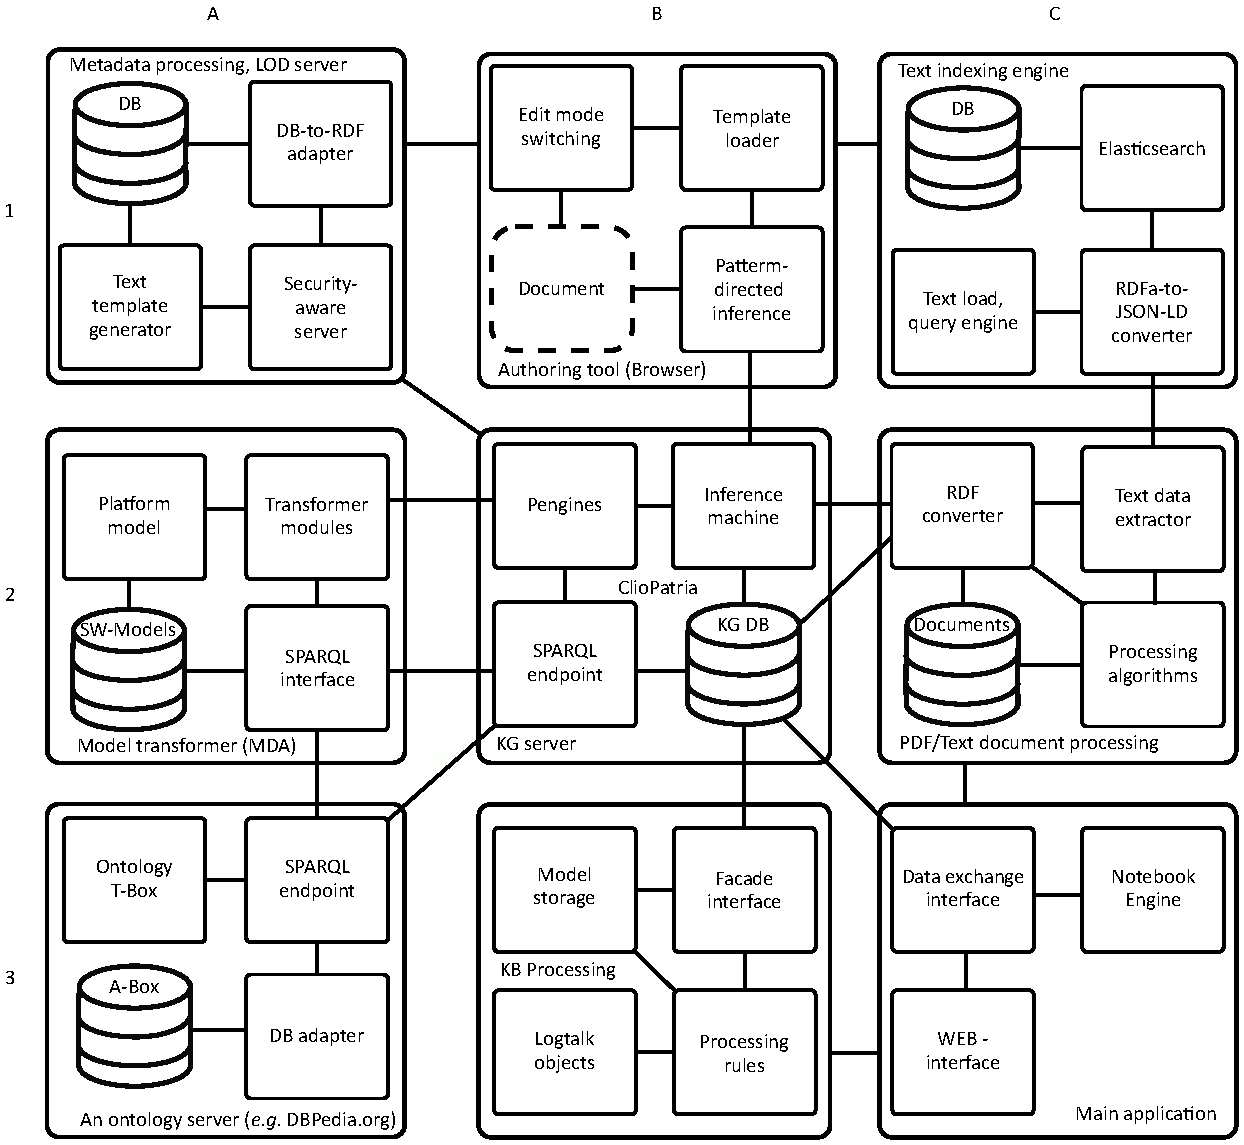
\includegraphics[width=1\linewidth]{architecture-mda-lod-ext-general.pdf}
    \end{column}
    \begin{column}{0.3\linewidth}
      \textbf{Abbreviations}\\[1ex]\scriptsize
      T-Module is Transformation module\\
      MDA is Model-Driven Architecture\\
      % CIM is Computationally Independent Model\\
      % PIM is Platform Independent Model\\
      % PSM is Platform Specific Model\\
      T-Box is Terminological Box\\
      A-Box is Instance Box\\
      % NGS is Next-Generation Sequencing\\
      KG DB is Knowledge Graph Database
    \end{column}
  \end{columns}
\end{frame}

\begin{frame}[fragile]
  \frametitle{Semantic web technologies \& Knowledge graphs}
  Semantic Web (WEB 3.0) is characterized with
  \begin{itemize}
  \item Technological basis, oriented to the web % User applications are always comprises interconnected distributed web-services.
  \item Standardized data formats, storage, and processing
  \item Open principles of data publishing
  % \item Knowledge Graph (KG) construction techniques
  \item Services for data storage and access provision
  \item Generalized and special user interfaces are used for data presentation\vspace{1em}
  \end{itemize}
%\end{frame}

% Knowledge graphs changed the aspects to the knowledge base as being a part of whole totality of knowledge, implying the obeying the global standards and techniques of its acquisition and processing.

%\begin{frame}
%  \frametitle{Knowledge Graphs}
For the Knowledge Graphs (KG), the following is of interest.
 \begin{itemize}
  \item Converged notions \textbf{data} and \textbf{knowledge} as something is \textbf{known}
  \item Contain data, relations, and metadata (vocabularies)
  \item Distinguished \textbf{node filling in} and \textbf{processing} graph triples, \emph{e.g.}, with SPARQL queries with UPDATEs
  \item Allow \textbf{postpone} the formal definition of a schema
  \item Three types of graph schemata: \textbf{semantic} (aimed at generalization), \textbf{validating} (\textbf{e.g.} semantics, \textbf{completeness} w.r.t. sets of relations), and \textbf{emergent} (infer a set of generalized structures and \textbf{reconstruct} the KG).
  \end{itemize}
\end{frame}

\begin{frame}[fragile]
  \frametitle{CPs PDF analysis}
  Meaningful information is the title and the code of the course, list of topics, distribution of study units (academic hours) between lectures, practice, seminars, personal work of student, list of questions for knowledge assessment, tests, \emph{etc}.
  \begin{enumerate}
  \item Convert PDF to XML by \texttt{Poppler}'s \texttt{pdftohtml -s -c -xml}
  \item XML is converted to in-object database of ordered \texttt{elements/5}
  \item Text bounding box by non-empty runs, excluding page numbers
  \item Line, run, font, page features assessment (indent, tail, numbers, \ldots) \label{cyb}
  \item Join runs in lines, lines in paragraphs, removing page breaks \label{cen}
  \item Recognition of sectioning, association of paragraph to sections
  \item Join and fold lists, assuming bullet lists have deeper level
  \item Data acquisition respecting sectioning, store them in a KG and an HTML file
  \end{enumerate}
  Steps \ref{cyb} and \ref{cen} are repeated until no joins were performed.\\[0.1em]

  Recognized KG data are filled in a Lua\LaTeX{} template using an MVC framework.

\end{frame}

\begin{frame}[fragile]
  \frametitle{Structure recognition}
  \begin{center}
    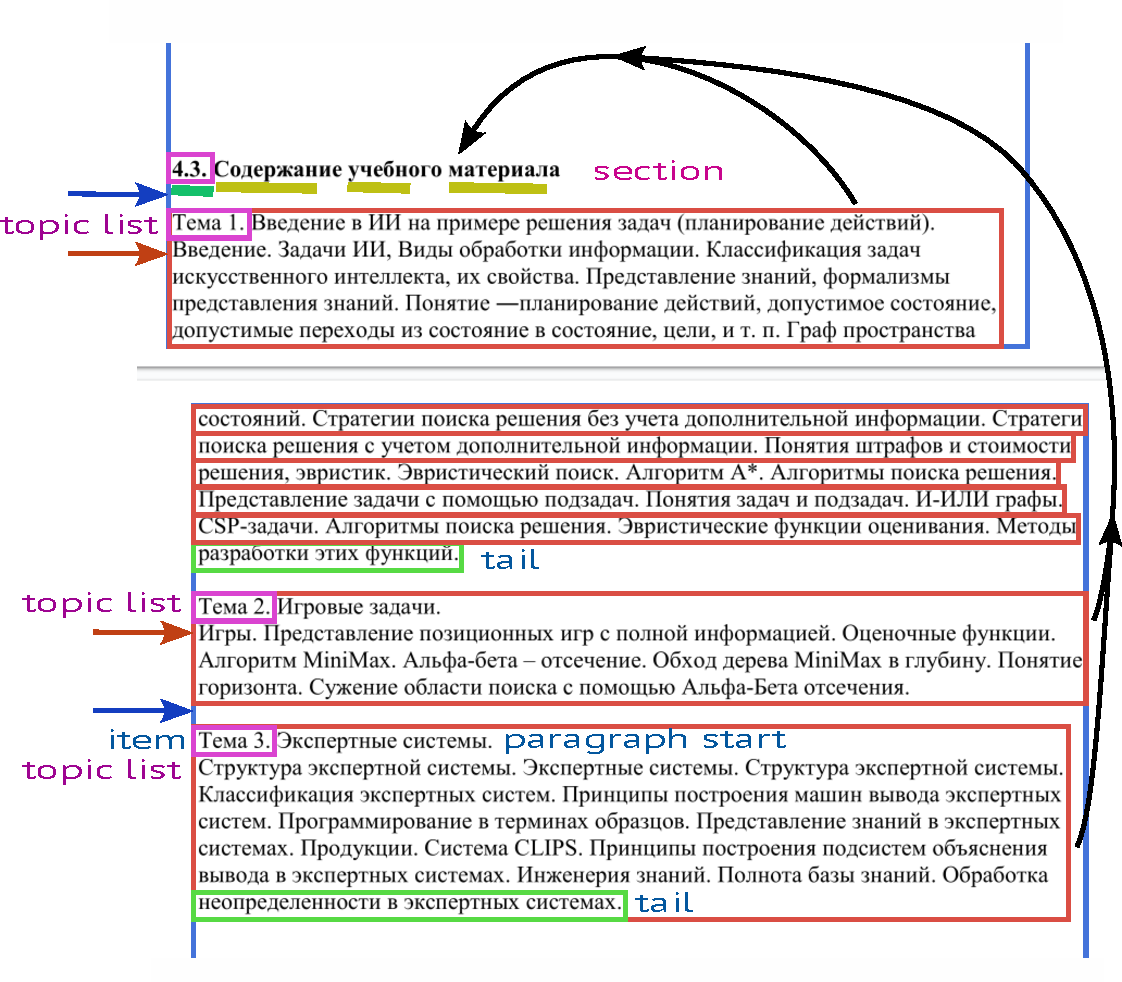
\includegraphics[width=0.8\linewidth]{paragraph-recognition.pdf}
  \end{center}
\end{frame}

\begin{frame}[fragile]
  \frametitle{CPs recognition scenario for IMIT, ISU}
\begin{minted}{logtalk}
:- object(CP_recognizer(_XML_, _HTML_File_Name_, _Document_IRI_),
          extends(as_db(_XML_)),  % A parametric object
          imports([CP_fonts, text_attrib, degraded, text_features,
                   CP_merge, text_CP_sections, gather_items,
                   CP_page_one, text_CP_fields, grouping,
                   htmlize])).    % Importing categories
   % . . . . . . . . . . . . .
   % Configuration parameters of the recognizer
   deviation(attributes, [10, 50]).    % tolerances
   deviation(paragraph, [50, 10]).     %
   deviation(parindent, [28]).         % 1 cm = 28 pt
   deviation(itemtextminlength, [10]). % The length of a "minimal item text".
   :- public(process/0).               % public predicate
   :- info(process/0, [ comment is 'Run all rules in an order' ]).
   process :-
      ::process_CP_fonts, !, ::process_attrs, !,
      ::process_degraded, !,       ::process_runs_merge, !,
      ::process_features, !,       ::process_merge, !,
      ::process_features, !,       ::process_merge, !,
      ::process_first_page, !,     ::process_CP_sections, !,
      ::process_item_gathering, !, ::process_merge, !,
      ::process_CP_fields, !,::process_grouping(ul), !,
      ::process_merge, !,          ::htmlize(_HTML_File_Name_, _Document_IRI_),
      !.
:- end_object.
\end{minted}
\end{frame}

\begin{frame}[fragile]
  \frametitle{Extending line-joining category}
\begin{minted}{logtalk}
:- category(CP_merge, extends(text_merge)).
    :- protected(lines_mergable/2).
    lines_mergable(A, B) :-  % Try to use default rules
        ^^lines_mergable(A, B), !. % Parent category predicate call
    lines_mergable(element(_, _, text, _, S1), element(_, _, text, _, S2)) :-
        ::gettext(S1, T1),    ::unterminated_sentence(T1),
        ::gettext(S2, T2),    ::cannot_start_sentence(T2), !.
    lines_mergable(element(_, _, text, A, _),  element(_, _, text, _, S2)) :-
        ::list_item(A),       ::gettext(S2, T2),
        ::cannot_start_sentence(T2), !.
    % . . . . . . .
    :- protected(unterminated_sentence/1).
    unterminated_sentence(T) :-
        re_match("[-/+=–—]\s*$", T, []).
    unterminated_sentence(T) :-
        string_lower(T, L),   re_match("url\s*:\s*$", L, []).
    % . . . . . . .
    :- protected(cannot_start_sentence/1).
    cannot_start_sentence(T) :-
        re_matchsub("^\s*[а-я]+\s*([):]?)", T, Dict, []),
        get_dict(1, Dict, ""), !.
    % . . . . . . .
:- end_category.
\end{minted}
\end{frame}

\begin{frame}
  \frametitle{Result}
  \begin{center}
    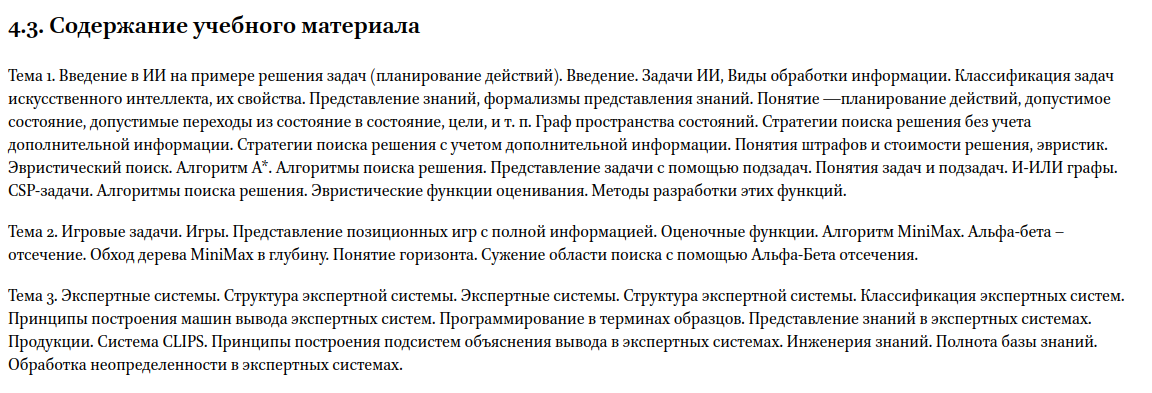
\includegraphics[width=\linewidth]{recognition-result.png}
  \end{center}
  For the \textbf{title} and \textbf{topics}, structures of KG graph are created, as well as \textbf{relations between them}, accounting contexts.
\end{frame}

\begin{frame}
\frametitle{``ISU Schedule'' Functions}
``ISU Schedule'' is a web-application has the following functions:
    \begin{itemize}
    \item[\faCogs] accounting main features of ISU institutions, such as:
        \begin{itemize}
            \item different timetables
            \item periodicity of classes
            \item time spending for classes variety
        \end{itemize}
        \item[\faEdit] editing of the education timetables for mural and extramural groups
        \item[\faSearch] printing schedules for an auditorium, course, faculty member, and student group
        \item[\faUserPlus] register a user
        \item[\faBirthdayCake] input holiday dates
        \item[\faDownload] load data from ``1С:University''
        \item[\faTable] schedule compilation with a genetic algorithm
    \end{itemize}

\end{frame}

\begin{frame}
    \frametitle{Administration panel}
    \begin{figure}[h!]
        \centering
        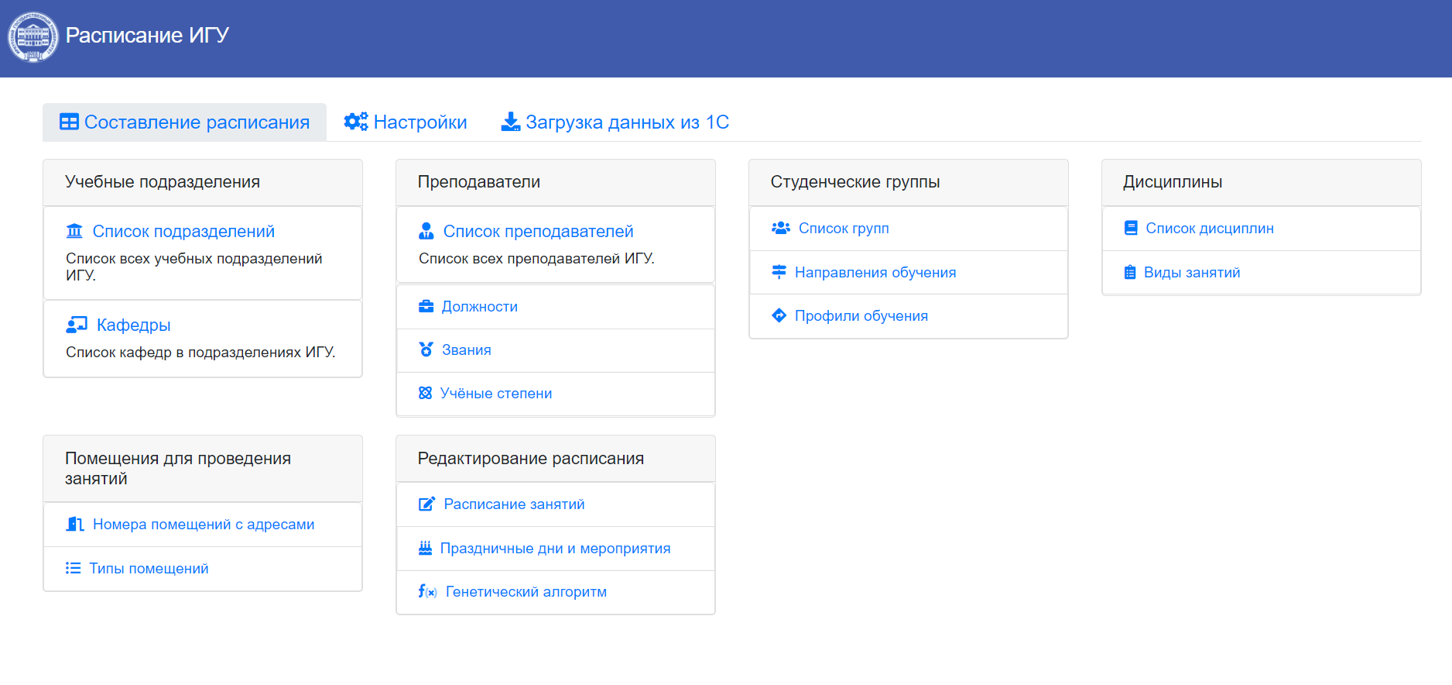
\includegraphics[width=1\textwidth]{img/panelAdmin.png}
    \end{figure}
\end{frame}

\begin{frame}
    \frametitle{A schedule view}

    \begin{figure}[h!]
        \centering
        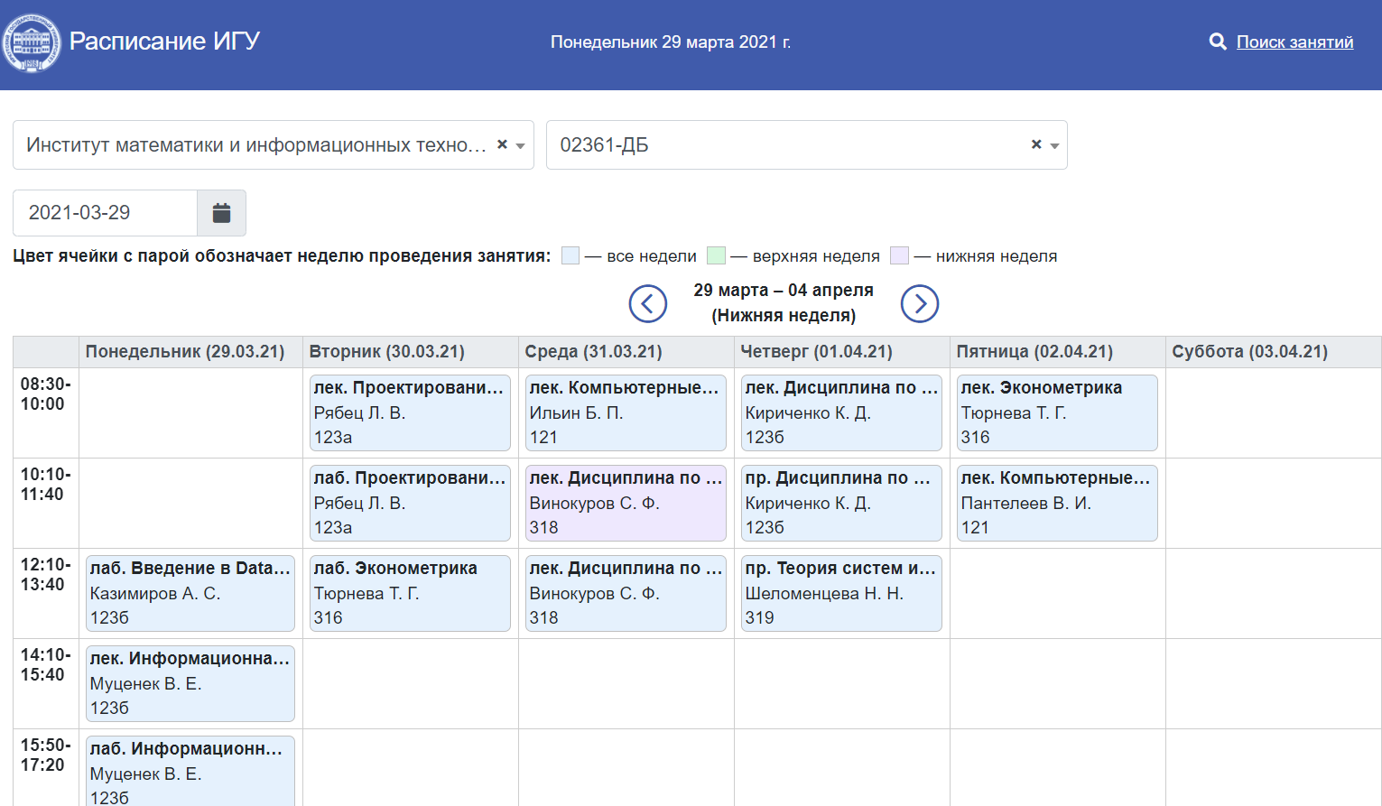
\includegraphics[width=1\textwidth]{img/viewSchedule.png}
    \end{figure}
\end{frame}

\begin{frame}
    \frametitle{Main program features}
    \textbf{Editing mode functions}
        \begin{enumerate}
            \item Adding classes for, a date, a time period, define periodicity
            \item Update class data:
            \begin{itemize}
                \item shifting a class to another day of week or a time period
                \item changing the auditorium
                \item assigning other teacher
            \end{itemize}
            \item Removing or cancellation of a class
        \end{enumerate}
  \textbf{Genetic algorithm} constructs a schedule for an institute, accounting
    \begin{itemize}
    \item teacher day load
    \item the capacity of auditoriums
    \item disabling gaps for student groups and faculty
    \end{itemize}
    \textbf{Program performance}

    \begin{itemize}
        \item[] For 30 student groups of IMIT, ISU
        \item An acceptable solution is obtained for 5000 iterations (40 minutes)
    \end{itemize}

\end{frame}

\begin{frame}
    \frametitle{A program execution result}
    \begin{figure}[h!]
        \centering
        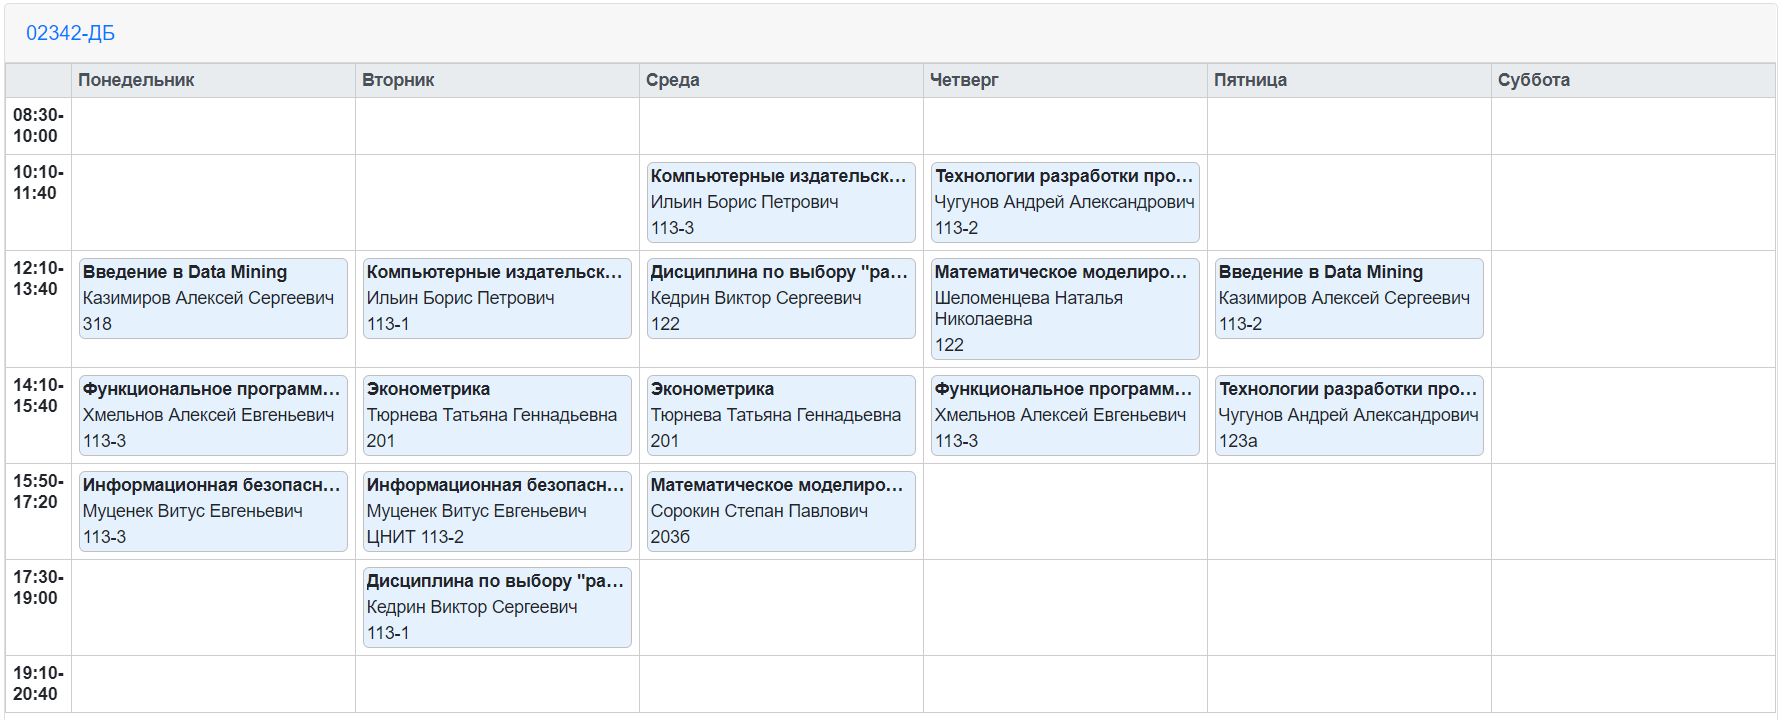
\includegraphics[width=1\textwidth]{img/geneticAlgorithm.png}
    \end{figure}
\end{frame}

\begin{frame}
  \frametitle{Conclusion}
  This is a progress report of R\&D of a Knowledge Graph based architecture and infrastructure for automation of creative activity of a faculty.  The following results were obtained:
  \begin{enumerate}
  \item Raw domain analysis, including, problem space
  \item Existing software and data source accounting
  \item Realized MVP-like utilities providing solutions of new problems
    \begin{itemize}
    \item Knowledge Graph (KG) component infrastructure is being organized
    \item Analyzing PDF-exported versions of CPs by a Logtalk knowledge-based system
    \item Collecting data from the CPs documents and store in KG
    \item Implementing verification software for parts of CP
    \item Document authoring tools are being implemented using generative approaches
    \item Techniques of Linked Open Data and standard vocabularies' usage is being formalized
    \end{itemize}
  \end{enumerate}
\end{frame}

\begin{frame}
  \begin{center}
  \Large Thanks for Your Attention!
\end{center}
\end{frame}




\end{document}

%%% Local Variables:
%%% mode: latex
%%% TeX-master: t
%%% End:
